This section presents the design exploration of a set of streaming applications being executed on a DMP.
The section describes how changing the thread mapping and core composition affect the benchmarks and what we can learn from this.
In addition, the impact of loop unrolling and how it helps exploit larger fused cores is investigated.

\subsection{Overview}

\begin{figure}
    \centering
    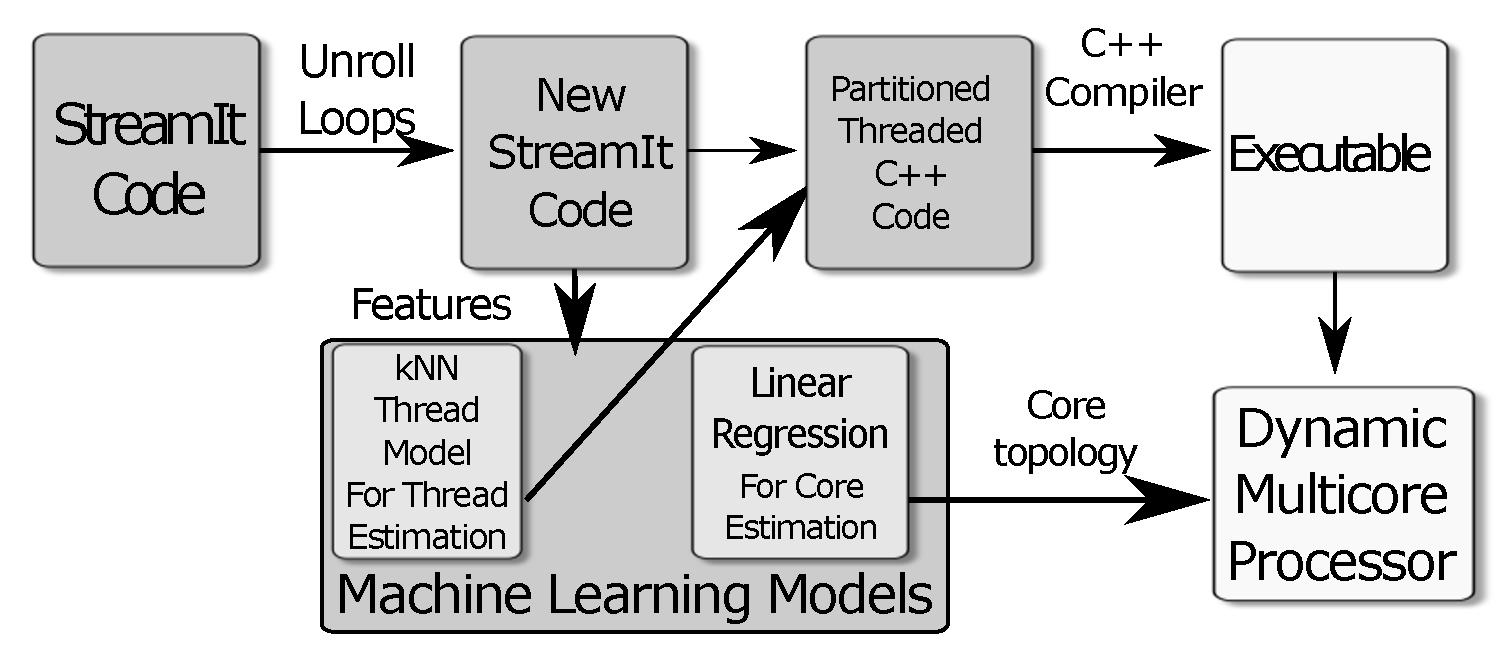
\includegraphics[width=1\textwidth]{streamit-paper/graphics/explanation.pdf}
    \caption{Description of the workflow.
    Two distinct machine-learning models are used to predict the optimal thread partitioning and core composition based on static code features.}
    \label{fig:overview}
\end{figure}

Figure~\ref{fig:overview} presents the workflow of the system used in this chapter.
First, the source-to-source StreamIt compiler is used to unroll loops as this is often beneficial when cores are composed as will be seen later in Section~\ref{core}.
Then, static code features such as the program's graph structure are extracted from the StreamIt code.
These features are used as an input to the first machine-learning model that determines the Thread Level Parallelism (TLP).
This information is used to partition the program into threads which is done by the StreamIt compiler which produces a C++ program using pthreads.
This C++ program is then compiled using the compiler for EDGE.

Then, a second machine-learning model is used which uses static code features extracted from the SteamIt code.
This model is used to decide on the core topology.
This is achieved by estimating the amount of Instruction Level Parallelism (ILP) that can be possibly extracted in each thread and by determining how many physical cores should be fused for that thread.
Finally, the processor is reconfigured to fuse the requested resources ahead of time and execute the partitioned program.


\subsection{Dynamic Multicore Processor}

%In this chapter the Dynamic Multicore Processor used for the research is based on an Explicit Data Graph Execution (EDGE) Instruction Set Architecture that resembles~\cite{sibi2014}.
%This differs from other DMPs such as CoreFusion, WidGET and Shared Architecture~\cite{ipek2007CoreFusion,Watanabe2010Widget,zhou2014sharingarch} which utilize a CISC/RISC instruction set.
To evaluate the work a customizable cycle-level simulator verified within 4\% of RTL is used.
The simulator is highly configurable, allowing the modelling of a variety of parameters such as the number of cores, details of the memory hierarchy and synchronisation schemes.
For the experiments in this chapter a 16 core dual issue configuration with 4 lanes per core, 16 KB private L1 caches and a 2 MB shared L2 is used.

\begin{figure}
    \centering
    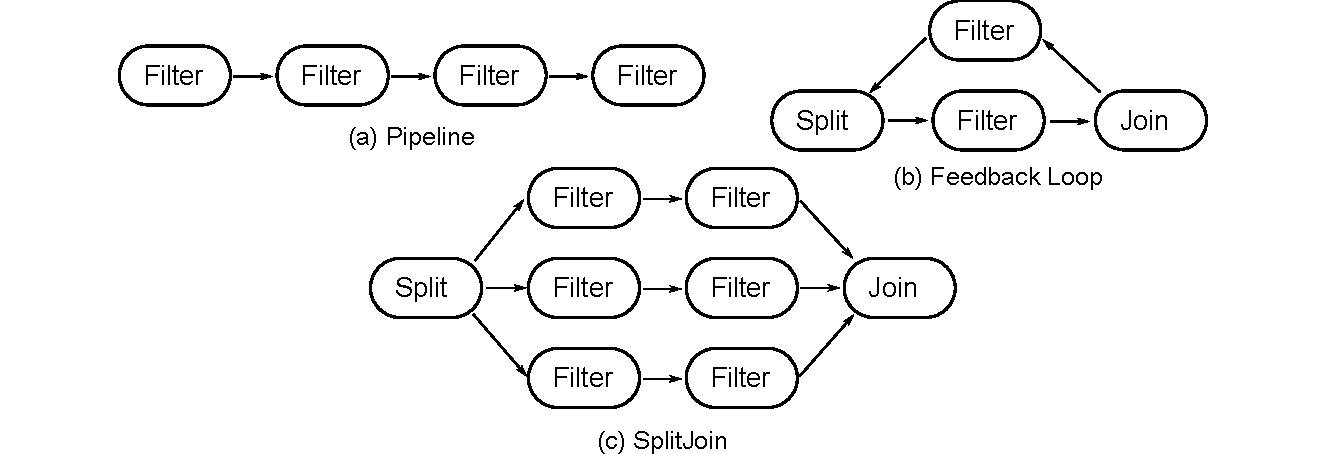
\includegraphics[width=1\textwidth]{streamit-paper/graphics/streamit_types.pdf}
    \caption{Visual representation of the three different StreamIt structures.}
    \label{fig:streamittypes}
\end{figure}
\subsection{StreamIt Benchmarks}

StreamIt is a high-level synchronous dataflow streaming programming language that defines programs as directed graphs.
StreamIt offers an elegant way of describing streaming applications, abstracting away how infinite data streams are managed to allow the programmer to solely focus on how the data must be treated.
A StreamIt program is composed of functions - called \textit{Filters} - which operate on streams of data.
Filters can be connected via \textit{Pipelines}, \textit{SplitJoins} or \textit{Feedback Loops}.

Figure~\ref{fig:streamittypes} displays the different methods of connections.
Pipelines (Figure~\ref{fig:streamittypes}(a)) represent a sequence of connecting filters operating on the same stream, each filter operating on the output of the previous filter.
In a SplitJoin (Figure~\ref{fig:streamittypes}(c)), data in the stream is passed through a split filter and either duplicated and passed on in parallel to the filters or distributed amongst the filters in a round-robin manner.
The output of all the filters in a SplitJoin are then concatenated in a round-robin fashion through a joiner filter.
Finally a Feedback Loop (Figure~\ref{fig:streamittypes}(b)) provides a way for filters to operate on their outputs.
The resulting program written in StreamIt represents a graph where the nodes are filters and their edges represent the incoming and outgoing data streams.

This chapter explores 15 StreamIt benchmark  all taken from the official StreamIt repository.
For each benchmark the default inputs provided in the repository are used and the default iteration count is set to 10. 

\subsection{Design Space}

The parameters and size of the space are given in table~\ref{tab:space}.
In this study all 16 cores are utilised; Core 0 is assigned to the main thread and for runtime management. 
This leaves 15 cores available for each application.
Each core is restricted to running only a single thread (no preemptive scheduling) which leads to a possible number of threads between 1 and 15.
Cores can be fused together to form a logical core with up to 15 physical cores, making the total number of cores assigned to a thread between 1 and 15.
This leads to a total space size of 32,767 unique combination per benchmark.

\begin{table}
\centering
\begin{tabular} { p{5.2cm}  p{1.8cm} }
      \toprule
      \textbf{Parameter} & \textbf{Values} \\ \midrule
      \# of cores in the processor & 16 \\
      \# threads per application & 1 -- 15 \\
      \# cores per thread & 1 -- 15 \\ \midrule
      \# sampled core compositions & 100 \\ 
      \# our sampled space & 1316 \\
      \# total sample space & 32762 \\ \bottomrule
    \end{tabular}
  \caption{Design space considered per application.}
  \label{tab:space}
\end{table}
\subsection{Sample Space}

\begin{figure}[h]
  \centering
    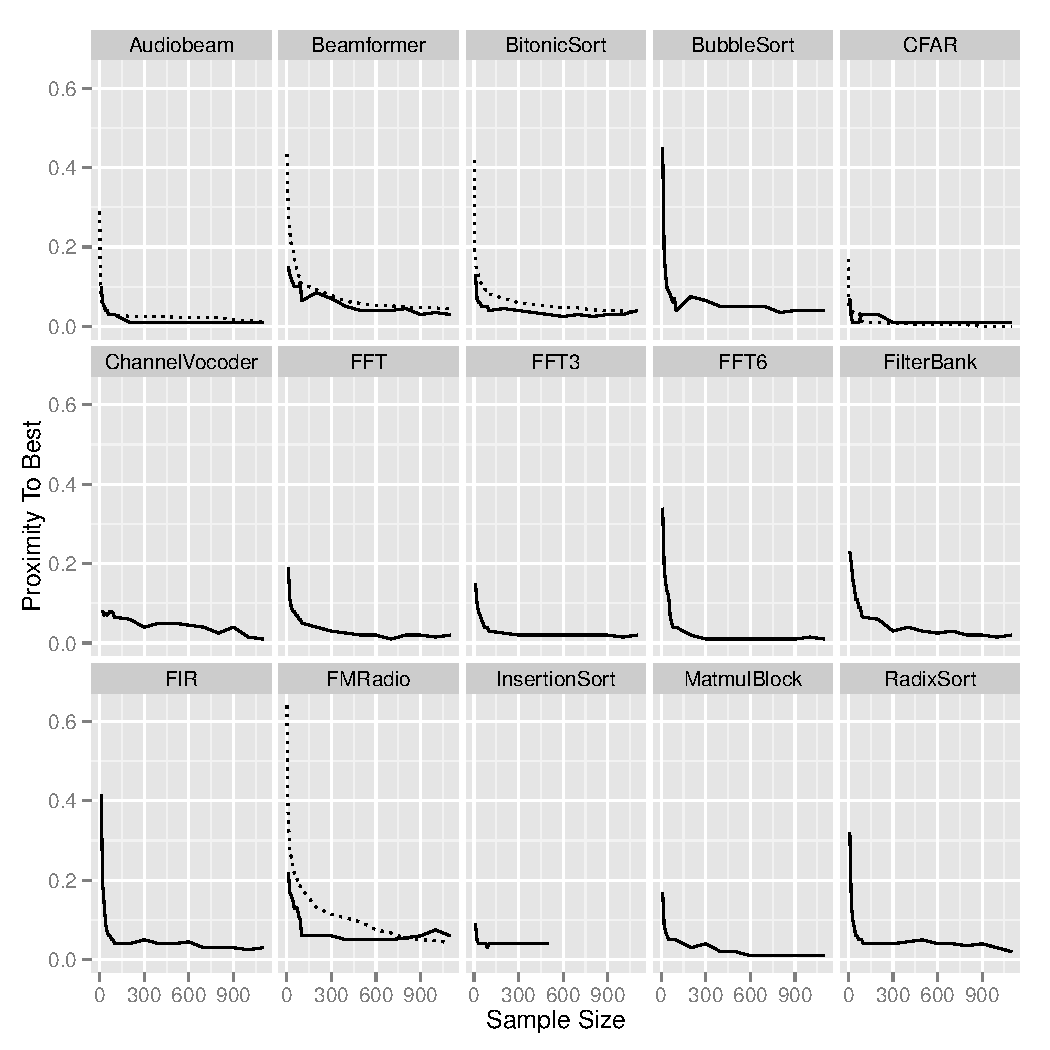
\includegraphics[width=1\textwidth]{streamit-paper/graphics/ESCProx.pdf}
    \caption{Statistical (plain line) and actual proximity (dotted line) to best performance using a subset of the sample space.}\label{fig:prox}
\end{figure}

\begin{figure*}[h]
 \centering
    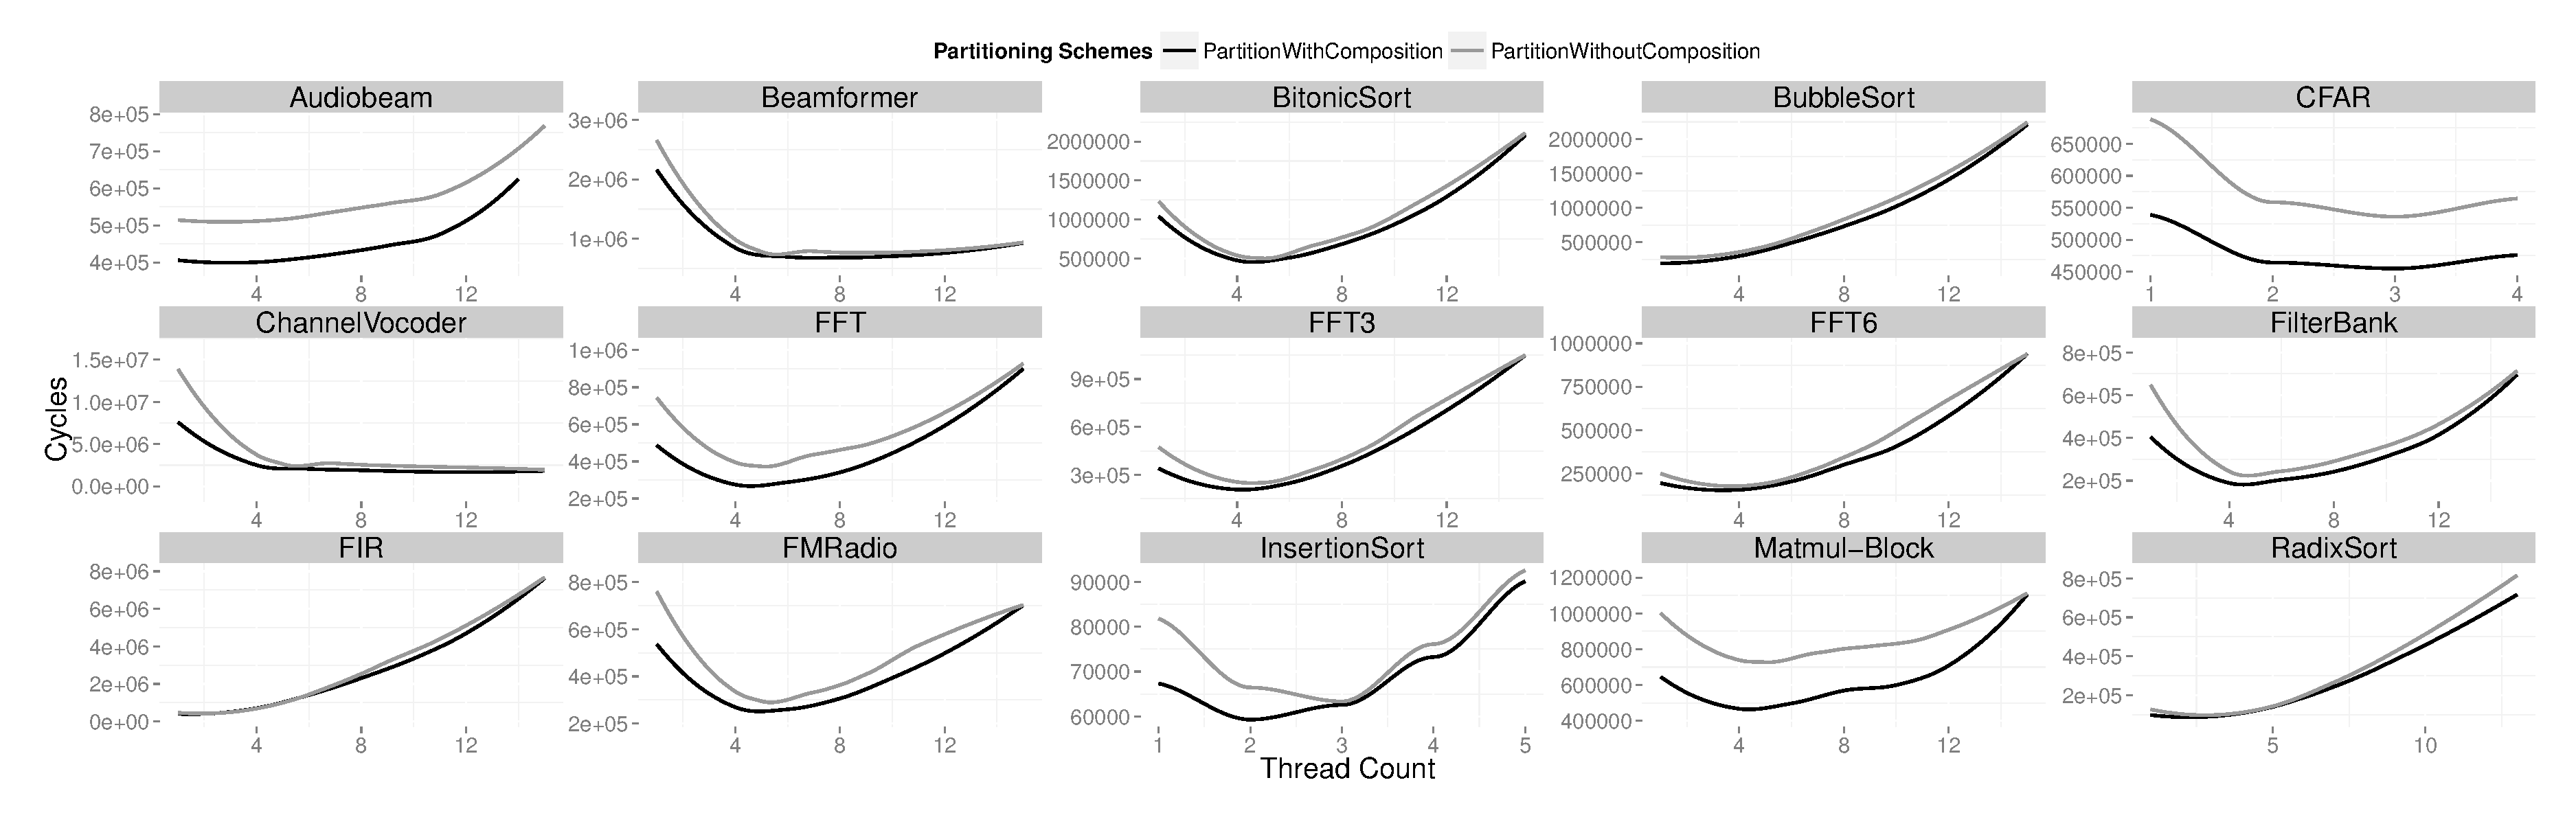
\includegraphics[width=1\textwidth]{streamit-paper/graphics/threadingmaybe.pdf}
    \caption{Performance as a function of the number of threads. The performance metric is number of cycles. Each benchmark has the performance measured with cores composed and with threads mapped to a single core.}\label{fig:threadtrend}
\end{figure*}
Given a partitioning, any benchmark that is split into 15 threads requires 32,767 executions to cover the entire space.
Running an exhaustive exploration of the space requires approximately a week of simulation on a 572+ node supercomputer.
For this reason, a sample of 1,316 random points from the entire space is utilised.
This roughly corresponds to 100 core compositions for each number of threads (the actual number, 1,316 is smaller than 1,500 since for low thread counts there are less than 100 possible different core composition).
\bench{InsertionSort} is the only exception since it can at most only be split into 5 threads leading to 415 sample points.

To gain confidence that the best configuration from the sample space is indeed close to the real best in the entire space, a statistical model based on the Stopping Criterion defined in~\cite{vuduc2003AutomaticPerf} is deployed.
This model estimates, given a sample of the total space, if the best observed performance of that sample space is within a percentage of the statistical best performance.
The results demonstrate that the sample space selected is representative of the whole space.

Figure~\ref{fig:prox} shows, for each of the benchmarks, the proximity to the statistical best when increasing the sub-sample space given a maximal uncertainty of 5\%  (\ie minimum 95\% confidence).
As can be seen by the plain line, the model shows that the best sample point is actually within 5\% (0.05 proximity) of the best for all benchmark.
To further prove that the statistical model based on the Stopping Criterion is indeed accurate, an exhaustive exploration of five benchmarks was conducted.
The dotted line in figure~\ref{fig:prox} shows the actual proximity to the best for \bench{Audiobeam}, \bench{Beamformer}, \bench{BitonicSort}, \bench{CFAR} and \bench{FMRadio}.
As can be seen after 1316 samples, the performance we achieve is actually very similar to the one predicted by the statistical model, hence confirming prior work~\cite{vuduc2003AutomaticPerf}.
To summarize, it can be concluded that the best point found in the sample space of 1,316 points is at least within 5\% of the real best in the exhaustive space with 95\% confidence.